% Configuration
\documentclass[11pt,a4paper]{article}
\usepackage[a4paper, top=2.0cm, bottom=2.0cm, right=2.0cm, left=2.0cm, nohead]{geometry}
\usepackage[utf8]{inputenc}
\usepackage{czech}
\usepackage{url}
\usepackage{graphicx}

% Disables some warning messages
\sloppy
\hbadness 10000

\begin{document}

% Header
\noindent
\begin{small}Dokumentace k projektu do předmětu PRL \\ 5.~dubna~2009\end{small} \\

% Title
\begin{center}
	\begin{large}\textbf{Pipeline Merge Sort}\end{large} \\
	\vspace{0.4cm}
	Petr Zemek \\
	\textit{xzemek02@stud.fit.vutbr.cz} \\
	\textit{Fakulta Informačních Technologií, Brno} \\
\end{center}

\section{Úvod}

Tato dokumentace popisuje algoritmus Pipeline Merge Sort a jeho implementaci
na architektuře PRAM. Je zde také diskutována teoretická časová složitost tohoto
algoritmu a zjištěné výsledky při vlastním experimentování s výsledným programem.

\section{Zadání, rozbor a analýza algoritmu}

Cílem projektu bylo implementovat algoritmus Pipeline Merge Sort \cite{1}.
Tento algoritmus využívá algoritmus Merge \cite{2}, který umí
seřadit dvě již seřazené posloupnosti do jedné. Obecně řazení na principu
spojování funguje tak, že se vstupní posloupnost nejdříve \uv{seřadí}
do posloupností o délce $1$, poté se všechny posloupnosti délky $1$ seřadí
do posloupnosti délky $2$, dále se tyto posloupnosti seřadí do posloupností
délky $4$ atd. Ve výsledku dostaneme seřazenou vstupní posloupnost. \\

\noindent
Algoritmus Pipeline Merge Sort (jak již název napovídá) využívá zřetězené zpracování,
kde posloupnost délky $n$ řadíme pomocí lineárního pole $log(n) + 1$ procesorů (pokud není $n$
mocnina dvou, pak je třeba vzít nejbližší vyšší hodnotu, která je mocninou dvou).
Každý z těchto procesorů má dvě výstupní fronty a první procesor má navíc ještě
vstupní frontu, kde jsou uloženy vstupní hodnoty. Na následujícím obrázku
je ukázka struktury pro délku vstupní posloupnosti $8$ (převzato z \cite{1}).

\begin{figure}[ht]
	\begin{center}
		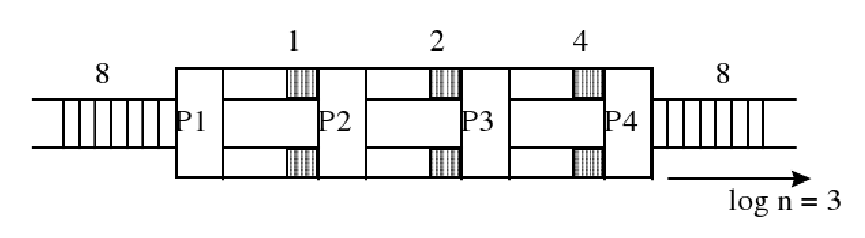
\includegraphics[width=8cm,keepaspectratio]{example}
	\end{center}
\end{figure}

\noindent
Zpracování funguje tak, že první procesor pouze střídavě rozhazuje hodnoty ze
vstupu do své výstupní fronty (první číslo do horní fronty, další do spodní atd.).
Druhý procesor vezme jedno číslo z horní fronty a jedno ze spodní fronty
a udělá z nich seřazenou dvojici, kterou umístí do své výstupní fronty (nejdříve do horní)
a poté si výstupní frontu prohodí (místo do horní bude v příštích krocích ukládat do spodní fronty).
Třetí procesor ze dvou seřazených posloupností délky $2$ vytvoří jednu seřazenou
posloupnost délky $4$ atd., až poslední procesor spojí dvě posloupnosti
délky $n / 2$ do výsledné seřazené posloupnosti. \\

\noindent
Každý procesor tedy spojuje dvě seřazené posloupnosti délky $2^{i-2}$, kde
$i$ je číslo procesoru. Procesor $P_{i}$ může začít zpracovávat hodnoty, když
má na jedné vstupní frontě (výstupní fronta předcházejícího procesoru)
posloupnost délky $2^{p-2}$ a na druhé frontě alespoň $1$ hodnotu, takže
začne $2^{p-2}+1$ cyklů po procesoru $P_{i-1}$.
Procesor $P_{i}$ tedy začne pracovat v cyklu $1 + \sum^{i-2}_{j=0}2^{j} + 1 = 2^{i-1} + i - 1$
a skončí v cyklu $(n - 1) + 2^{i-1} + i - 1$ \cite{1}. \\

\noindent
Algoritmus skončí za $n + 2^{log(n)} + log(n) - 1 = 2n + log(n) - 1$ cyklů, tedy
časová složitost je $t(n) = O(n)$ (lineární). Jelikož počet procesorů
je $p(n) = log(n) + 1$, tak cena $c(n) = t(n)\cdot p(n) = O(n)\cdot O(log(n)) = O(n\cdot log(n))$,
je optimální \cite{1}.

\section{Postup řešení pro PRAM}

Každý procesor má dvě výstupní fronty, horní a spodní, každá má z důvodu jednoduchosti
velikost podle počtu řazených položek. Všechny horní fronty jsou uloženy v jednom
poli, ve kterém se indexuje podle čísla procesoru vynásobeném počtem řazených prvků.
Kromě těchto front si u každého procesoru uchovávám aktuální frontu, do které
dává svůj výstup, kde je konec u dané fronty, kolik znaků bylo z každé fronty
přečteno a aktuální počet zpracovaných prvků. Dále je u každého procesoru příznak,
zda může začít přehazovat (a řadit) vstupní hodnoty na výstup. \\

\noindent
Index začátku fronty pro daný procesor získávám ve funkci \texttt{getProcQIdx},
který se vypočte jako $(p - 1) * n + 1$, kde $p$ je číslo procesoru a $n$ je
počet řazených hodnot. Pro práci s frontami jsem si vytvořil následující funkce.
Funkce \texttt{isEmptyQ} zjišťuje, zda je fronta prázdná, funkce \texttt{isFullQ}
zjišťuje, zda je fronta plná a nic do ní nelze zapsat, funkce \texttt{putValueToQ}
vloží zadanou hodnotu do fronty, funkce \texttt{getFrontItemQ} vrací
položku z čela fronty (ale neodstraní ji -- to dělá až funkce \texttt{removeFrontItemQ}).
Poslední funkce pro práci s frontami je \texttt{swapOutQ}, která prohodí frontu,
do které daný procesor aktuálně zapisuje svůj výstup. \\

\noindent
V hlavním programu je vnější smyčka, která jde od $1$ do $2*n + log(n) - 1$,
kde $n$ je počet řazených hodnot (resp. nejbližší druhá mocnina k této hodnotě,
viz analýza algoritmu), což je počet kroků algoritmu. Poté následuje
paralelní cyklus, kde (kvůli synchronizaci procesorů při čtení, resp. zápisu do front)
provedou svou činnost nejdříve všechny liché procesory a poté pracují všechny sudé procesory.
Tento způsob synchronizace má za následek pouze zdvojnásobení časové složitosti
vnitřní části cyklu a tedy nemá vliv na řád časové složitosti. \\

\noindent
První procesor pouze střídavě dává hodnoty ze vstupu na své výstupní fronty.
Každý procesor může začít zpracovávat hodnoty až po tom, co má na jedné frontě
kompletní seřazenou posloupnost a na druhé frontě alespoň jednu hodnotu.
Pokud daný procesor přečetl (a zapsal do své výstupní fronty) požadovaný počet
hodnot, dojde k přehození výstupní fronty (z horní na dolní a naopak).
Každý procesor si musí hlídat, kolik hodnot už přečetl z které fronty, aby nezačal
číst z následující posloupnosti, což by vyústilo ve špatně seřazený vstup. \\

\noindent
Výsledná seřazená posloupnost je po skončení vnějšího cyklu k dispozici v horní
frontě posledního procesoru.

\section{Použití programu}

Program očekává (na standardním vstupu) jako první číslo počet řazených položek
a poté hodnoty k seřazení.
Pokud tedy například chci seřadit 5 hodnot 1-5, tak na vstupu musí být zadáno
\texttt{5 1 2 3 4 5}. Po seřazení položek je seřazená posloupnost vytištěna na
standardní výstup.

\section{Experimenty}

V rámci praktického experimentování s programem jsem provedl sadu testů,
jejichž výsledky zde předkládám. V následující tabulce je vždy uveden
počet řazených položek a celkový čas řazení. Položky byly generovány náhodně
a pro zmírnění nepřesnosti měření proběhlo každé měření desetkrát a jako
výsledná hodnota byl zvolen průměr.

\begin{center}
	\begin{tabular}{| l | l |}
	\hline
		Počet prvků & Celkový čas (s) \\
	\hline
		100 & $2.2$ \\
		200 & $5.4$ \\
		300 & $11.5$ \\
		400 & $16.2$ \\
		500 & $19.6$ \\
		600 & $24.6$ \\
		700 & $29.0$ \\
		800 & $35.3$ \\
		900 & $40.2$ \\
		1000 & $46.8$ \\
	\hline
	\end{tabular}
\end{center}

\noindent
Následující graf zobrazuje potřebný čas v závislosti na počtu řazených položek.

\begin{figure}[ht]
	\begin{center}
		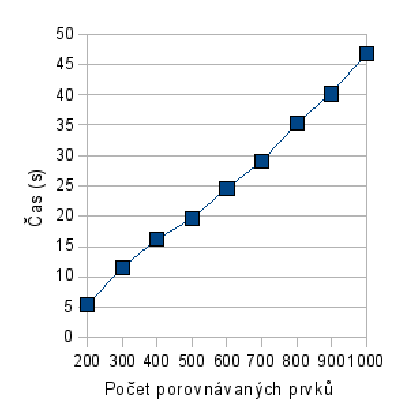
\includegraphics[width=5.0cm,keepaspectratio]{graph}
	\end{center}
\end{figure}

\noindent
Z grafu jde názorně vidět, že nárust času vzhledem k velikosti instance je
lineární, což odpovídá časové složitosti zjištěné při teoretické analýze algoritmu.

\section{Závěr}

Během vypracování projektu byla dodržena všechna specifika daná zadáním.
Projekt byl úspěšně otestován na školním serveru \texttt{merlin.fit.vutbr.cz}
pomocí vlastního testovacího scriptu.

\subsection*{Metriky}

\noindent
Počet zdrojových souborů: 1 \\
Počet řádků kódu: 397 (bez prázdných řádků, včetně komentářů)

\begin{thebibliography}{77}
\small
\bibitem{1} Hanáček P., Přednášky do předmětu PRL, \url{https://www.fit.vutbr.cz/study/courses/PDA/private/}, [citováno 5.4.2009]
\bibitem{2} Merge algorithm, Wikipedia - the free encyclopedia, \url{http://en.wikipedia.org/wiki/Merge_algorithm}, [citováno 5.4.2009]
\end{thebibliography}

\end{document}
